% Template for ICASSP-2016 paper; to be used with:
%          spconf.sty  - ICASSP/ICIP LaTeX style file, and
%          IEEEbib.bst - IEEE bibliography style file.
% --------------------------------------------------------------------------
\documentclass{article}
\usepackage{spconf,amsmath,graphicx,bm,setspace}
\usepackage{todonotes}
\setlength{\marginparwidth}{1.5cm}
\usepackage{lipsum}
\usepackage{graphicx}
\graphicspath{{images/}}

% ADD THE FOLLOWING COUPLE LINES INTO YOUR PREAMBLE
\let\OLDthebibliography\thebibliography
\renewcommand\thebibliography[1]{
  \OLDthebibliography{#1}
  \setlength{\parskip}{0pt}
  \setlength{\itemsep}{0pt plus 0.3ex}
}

% Example definitions.
% --------------------
\def\x{{\mathbf x}}
\def\L{{\cal L}}

% Title.
% ------
\title{A Knowledge Transfer and Boosting Approach to the Prediction of Affect in Movies}
%
% Single address.
% ---------------
\name{Sabyasachee Baruah$^o$, Rahul Gupta$^+$, Shrikanth Narayanan$^+$}
\address{$^o$Indian Institute of Technology, Kharagpur, West Bengal, India \\
$^+$Signal Analysis and Interpretation Lab, University of Southern California, Los Angeles, CA, USA}  
\begin{document}
\ninept
%
\maketitle
%
\begin{abstract}
   Put abstract here 
 
\end{abstract}
%
\begin{keywords}
Gradient Boosting, Knowledge Transfer, Valence, Arousal
\end{keywords}
%
\section{Introduction}
\label{sec:intro}

\section{Background}


\section{Dataset}
%The data is taken from the LIRIS-ACCEDE(Annotated Creative Commons Emotional DatabaseE for affective video content analysis) database \cite{baveye2015liris} presented in the 2016 MediaEval Emotional Impact of Movies Task. The dataset contains 30 short films of length varying from 3 to 28 minutes, each with a valence and arousal label in the range -1 to 1 for every second, annotated by 10 participants.

We use the {\it Annotated Creative Commons Emotional DatabaseE for affective video content analysis} (LIRIS-ACCEDE) dataset for the purpose of our experiments.
This dataset was also used as part of the {\it emotional impact of movies task} organized at the MediaEval challenge 2016 \cite{}.
The dataset consists of 30 short films of length varying from 3 to 28 minutes.
A set of ten annotators rate each movie for the affective dimensions of arousal and valence at a frame rate of 1 sample per second within a range of -1 to 1. 
For further information regarding the dataset, we refer the reader to \cite{}.
In the next section, we describe the features used in our experiments.

\subsection{Feature extraction}
We use an assembly of visual, speech and music features to train our models.
Table \ref{table:features} shows the list of features along with their frame rate and toolbox used. 
Note that the frame rates of features from different sources are different.
In order to synchronize the features with the annotations, we extract statistics on the features along a temporal window with a shift of 1 second. 
We extract a set of nine statistics (mean, median, standard deviation, kurtosis, lower and upper quartile, minimum, maximum and range) for every feature. 
Figure \cite{} depicts the extraction of these statistics on the features.
We chose the length of the temporal windows as the one that maximizes the mutual information between the computed features and affect labels (available on the training set). 

\begin{table}[t]
\centering
\begin{tabular}{|@{}l@{}|r|r|r@{}|}
\hline
{\bf Source} &{\bf Features} & {\bf FPS} & {\bf Toolbox} \\ \hline
Visual & Luminance, intensity & 30 & OpenCV \\ 
       & and optical flow & & \cite{} \\ \hline
Audio & Mel-frequency cepstral coefficients,& & \\
               & coefficients, voicing probability, & & \\  
               & harmonic to noise ratio, zero crossing & 100 & OpenSmile \\  
               & rate, crossing rate, fundamental & &\cite{} \\  
               & frequency, log energy & & \\ \cline{1-2}
Music & Chroma features (12 semitones) & & \\ \hline
\end{tabular}
\caption{List of features}
\label{table:features}
\end{table}


%\begin{figure}[t]
%\centering
%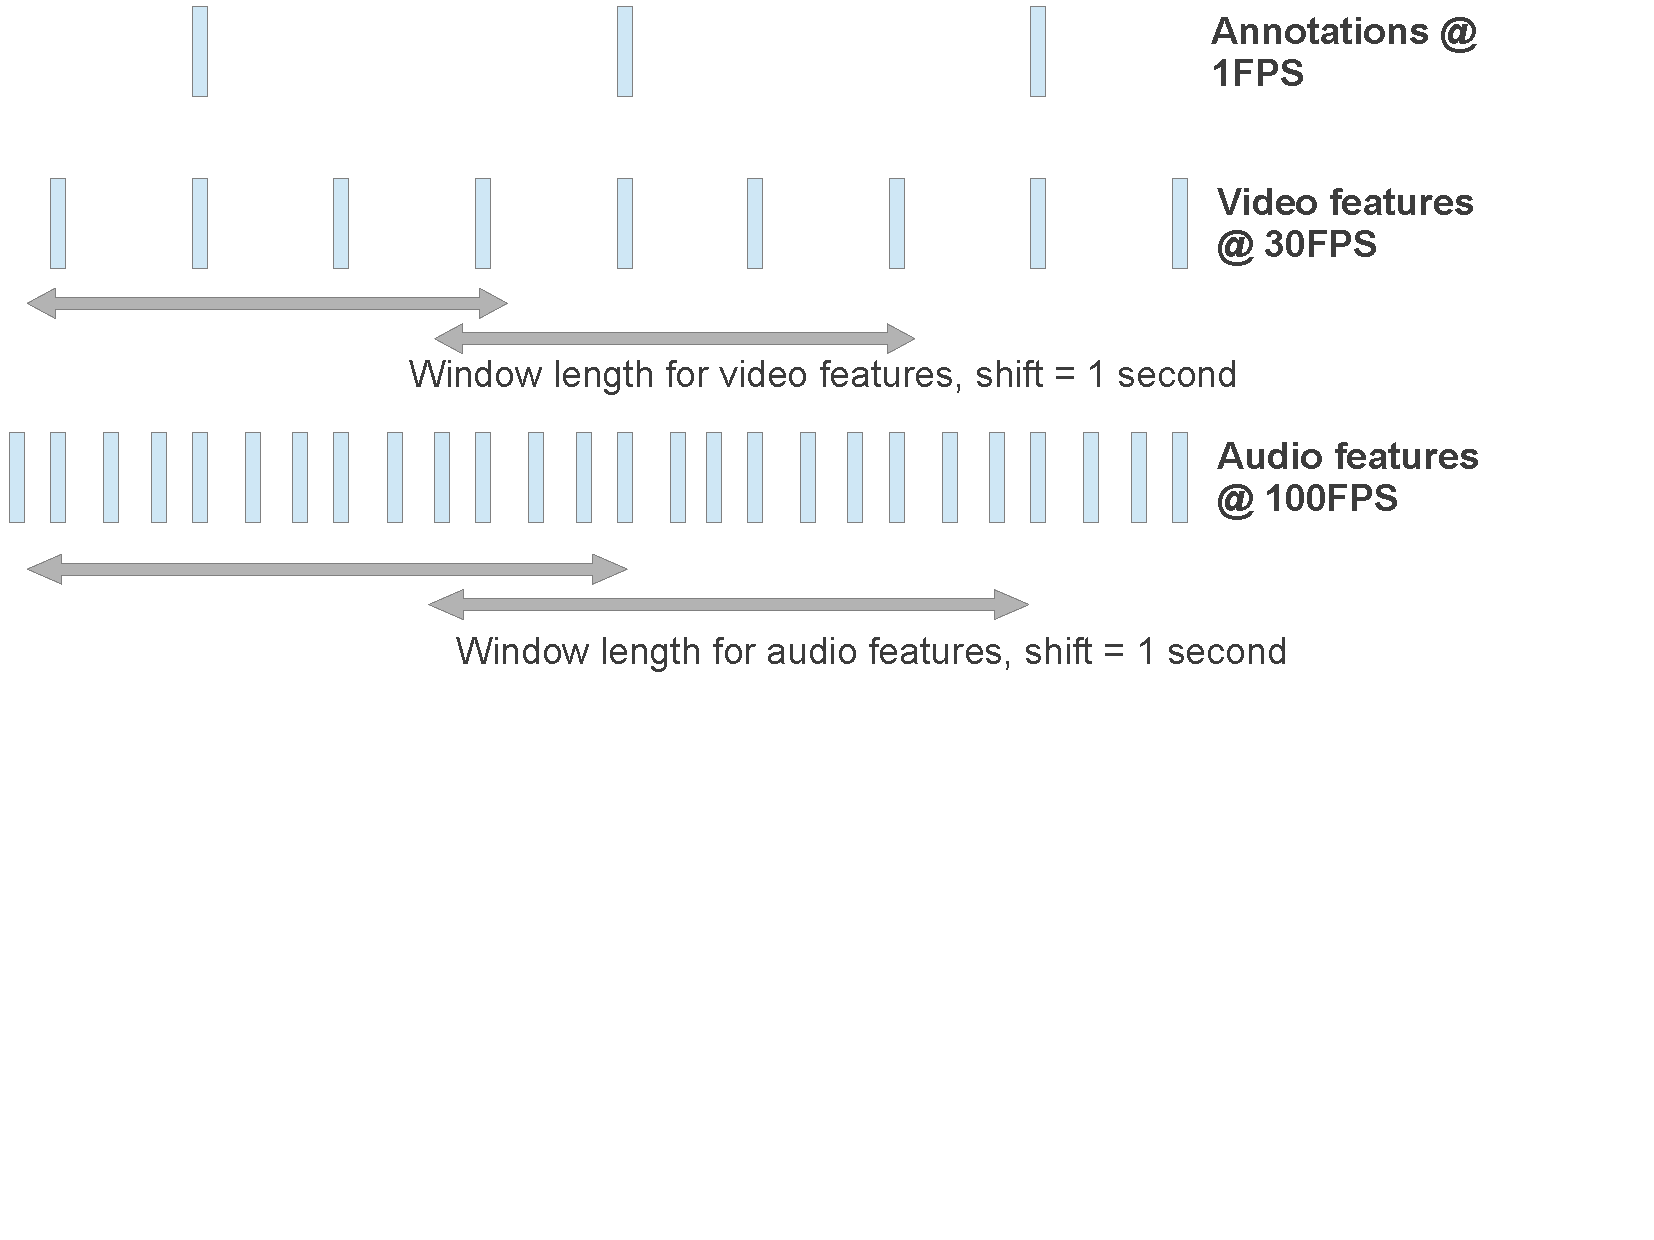
\includegraphics [trim=0cm 10cm 3cm 0cm,clip=true,scale=.355] {images/features_fig.pdf} 
%\caption{}
%\label{back_fig}
%\end{figure}


%\indent  A variety of visual, speech and music features are used for training our model. The visual features used are luminance, intensity and optical flow. The speech features are mel-frequency cepstral coefficients, voice probability, zero crossing rate, harmonic to noise ratio, fundamental frequency and energy logarithm. We also include the first and second derivative, and the arithmic mean and standard deviation of the countour of the signal for every speech feature. Lastly we compute 12 semitones for our musical chroma features. We have used the OpenSMILE toolbox for feature extraction. A total of 9 statistics - mean, median, standard deviation, kurtosis, lower and upper quartile, minimum, maximum and range are computed for every feature. We choose a 10 second wide sliding window for calculating our statistics. In total we have 156 visual, speech and musical features, each with nine statistics, thus ending up with a dimension of 1404 for our feature matrix.

\section{Methodology}

We test several regression schemes to predict the continuos valence and affect ratings from the features described in the last section.
Initially, we establish a baseline using multiple regressors.
We discuss the performance of the baseline models and motivate our knowledge transfer and gradient boosting based method.
All our experiments are performed by using a leave one out cross-validation scheme.
During cross-validation, we use 25 movies as the training set, 4 for validation and 1 movie in the test set.
The primary metric for the evalauation of our methods is Concordance Correlation Coefficient (CCC) \cite{} between the annotated ground truth and the predicted ratings on the test set.
This metric accounts for both the similarity of pattern between the two time series as well as the difference of bias between them. 
Along with this, we also report the correlation coefficient and the Root Mean Square Error (RMSE) between the predicted and the true ratings.
In the next section, we describe the baseline models.

\subsection{Baseline}
%The features and annotations are available at different time frequencies. The video and audio features have been extracted at a rate of 30 and 100 values per second respectively, whereas the ground truth is annotated for each second. To align both these sequences together, we calculate the aforementioned nine statistics over a sliding window on the feature array and assign the computed feature vector of dimension 1404 to the time second at the center of the window. Concordance correlation coefficient is employed as the evaluation metric. We observe the variation in performance for different models on baseline performance as shown in tables \ref{Valence_table} and \ref{Arousal_table}. 

%Farther analysis of the performance of the baseline models shows the variation in performance across the movies, as shown in figure. The movies in our dataset span a wide variety of genres (figure) and enough training data is not available for each type of movie. One of the examples is the film, \textit{To Claire From Sonny}, which is the only romantic movie in the dataset and thus doesn't match any of the movies in the training set in genre, leading to inaccurate predictions of valence and arousal (shown in the figure). To overcome this problem we require a much larger dataset that should have enough variation to be representative of the different genres of the LIRIS-ACCEDE dataset, but should also be compatible so that the knowledge gathered (trained model) can be used to predict the affective labels in the original dataset.

%To this affect we make use of the Discrete LIRIS-ACCEDE dataset. It contains 9800 short video clips of length 8-12 seconds. The clips have been taken from 160 movies. The ground truth consists of a single global valence and arousal label, unlike the previous dataset, in the range 1 to 5, annotated by 1517 annotators from 89 different countries using crowdsourcing. The differences are shown in table \ref{differences}.

%\indent Farther analysis of the performance of the baseline models shows the variation in performance across the movies, as shown in figure \ref{comparison}. The movies in our dataset span a wide variety of genres (figure \ref{genre}) and enough training data is not available for each type of movie. One of the examples is the film, \textit{To Claire From Sonny}, which is the only romantic movie in the dataset and thus doesn't match any of the movies in the training set in genre, leading to inaccurate predictions of valence and arousal (shown in the figure \ref{comparison}). To overcome this problem we require a much larger dataset that should have enough variation to be representative of the different genres of the LIRIS-ACCEDE dataset, but should also be compatible so that the knowledge gathered (trained model) can be used to predict the affective labels in the original dataset.

We use a set of three regressors (linear regression, ridge regression and neural network) to predict the affect ratings from the features. 
Linear regression \cite{} is the simplest of the three regressors and linearly maps the features to the affect ratings.
Like linear regression, ridge regression \cite{} also performs a linear mapping.
However the weights for ridge regression are regularized \cite{}, a scheme helpful in cases involving limited amount of training data.
We test two version of these schemes: with and without feature selection.
During feature selection, we remove features with absolute value of the correlation coefficient below a certain threshold (tuned on the development set).
Correlation coefficient quantifies the linear relationship between the features and the ratings, therefore removal of features with a low correlation coefficient can potentially boost the performance of linear models such as linear and ridge regression. 
Finally, neural networks perform a non-linear mapping between the features and the affect ratings. 
We train a neural network with one hidden layer.
The number of neurons is tuned on the development set and they have a sigmoidal activation.
We do not perform feature selection with neural networks ???.
Table \ref{} shows the results for the performance of these three baseline regression models. 


\subsubsection{Discussion} From the results, we observe that the performance for affect prediction varies across the three models.
Particularly, the best performing models are different for the two dimensions.
Neural network regressor performs the best for valence, while linear regression with feature selection performs the best for arousal.
We further list the performances for each movie as obtained using the best regressors for both arousal and valence in Figure~\ref{}. 
The figure shows that the performance per movie varies quite a bit, thereby indicating that a model trained on a limited amount of dataset may not generalize well.
For further analysis, we show the histogram of movie genre distribution in the LIRIS-ACCEDE dataset in Figure~\ref{}.
We observe that certain genres are poorly represented in the dataset, for instance, romance.
This is also reflected in our results as the trained models do not perform well on the romantic movies (marked with a $\xi$ in the figure). 
Our analysis reflects that a large diversity in the set of movie genres and their limited representation in our dataset needs to be addressed.
We propose a knowledge transfer + gradient boosting methodology to address this problem, as is discussed in the next section.

\begin{table}[t]
\centering
\begin{tabular}{|l|p{2.2cm}|p{2.2cm}|}
\hline
				& Continuous LIRIS-ACCEDE	& Discrete LIRIS-ACCEDE \\ \hline
Duration			& 3 - 28 minutes			& 8 - 12 seconds		\\ \hline	
Global/Continuous	& Continuous				& Global 				\\ \hline
Range			& -1 to 1					& 1 to 5				\\ \hline
\end{tabular}
\caption{Differences between Continuous LIRIS-ACCEDE and Discrete LIRIS-ACCEDE.}
\label{differences}
\end{table}

\subsection{Proposed method}
As observed from the results and analysis in the previous section, we need to address the problem of limited data leading to poor generalization of our models.
In this section, we propose a knowledge transfer combined with a gradient boosting approach to address the aforementioned issue.
During knowledge transfer, we borrow information learnt on a larger (albiet mismatched) dataset for affect prediction on the dataset of interest (LIRIS-ACCEDE).
This is followed by gradient boosting, where we combine models learnt on the LIRIS-ACCEDE with the existing knowledge transfer models.
We discuss these proposed models in detail below. 

\subsection{Knowlege Transfer (KT)}
During Knowledge Transfer (KT), we train models on a another dataset and operate them on the LIRIS-ACCEDE dataset to obtain the affect ratings.
To this effect, we use the {\it Discrete LIRIS-ACCEDE dataset} consisting of a larger set of ~10k movie clips.  
The discrete LIRIS-ACCEDE dataset is different from the continous LIRIS-ACCEDE dataset in several respects.
The discrete dataset consists of small movie clips (~10 seconds in length) as opposed to the continous dataset (3-28 mins in length).
Furthermore, the annotations are provided at the global scale with a single valence and arousal rating for each clip.
The annotations are in the range of 1-5 as opposed to the scale of -1 to 1 in the continous dataset. 
We describe the model training on the discrete dataset and application on continous dataset in detail below.

\subsubsection{KT model training}
Initially, we extract the same of set of features on the discrete dataset as mentioned in the Table~\ref{}.
However, we compute the statistics (listed in section~\ref{}) over the entire duration of the clip.
We then train a ridge regression model on the feature statistics to predict the discrete ratings.

\subsubsection{KT model application}
In order to apply the model trained on the discrete dataset, we again use the feature assemble in Table~\ref{}.
However the feature statistics are computed over a fixed window length of 10 seconds with a shift of 1 second (please refer to Figure~\ref{}). 
This window length is emperically chosen to match the length of clips in the discrete dataset.
We then predict the affective dimensions per second using the model trained in the last step.
Since the annotation scales are different for each dataset, we chose to linearly scale the ratings predicted by the knowledge transfer model.
We obtain the predictions using the KT model on the training set and linearly scale them such the minimum mean sqaured error between the KT model predictions and the true ratings is minimized. 
After the KT step, we train a gradient boosting model as discussed in the next section. 

%We extract the same set of features for the short video clips of Discrete LIRIS-ACCEDE as we had done for the movies of Continuous LIRIS-ACCEDE. We train a model on the 9800 videos and predict single values of valence and arousal for each second for the movies. To scale the predictions from the range $[1,5]$ to $[-1,1]$, we use linear modeling by minimizing the squared error between the true labels and predictions. 

\subsection{Gradient boosting (GB)}
%We have used the knowledge gathered from the videos of Discrete LIRIS-ACCEDE to predict the labels of a different dataset, Continuous LIRIS-ACCEDE. However the huge difference in duration between the video clips and movies means that the model cannot still account for the effect of past scenes on the emotions felt by the viewer at the moment. Knowledge transfer predicts the sequence of labels based only on the feature vector of the corresponding second. We leverage the features of the movies to take care of the effect of history while experiencing emotions in viewing a movie.

%We calculate the pseudo-residual error, the difference of the predictions of knowledge transfer and the ground truth. This difference sequence becomes our new target and we train a model on the feature matrix of the movies to predict it. To account for the effect of history on the current annotation of valence and arousal, we shift our feature matrix forward in time relative to the target vector. The delay is found out by maximising mutual information between the shifted feature matrix and target vector. We additionally apply a smooting average filter on our predictions to subtract any noise present in the movie features. We add our predictions of the pseudo-residual error to the output of knowledge transfer to get our new predictions. This process is repeated again until we no longer see an improvement in performance.

The goal of GB model is to extract information from the smaller set of continuous LIRIS-ACCEDE dataset and {\bf add} it to the prediction from the KT model.
We use the gradient boosting approach similar to the one proposed by Gupta et al. \cite{} for our experiments.
Gupta et al. \cite{} proposed an appraoch using linear filters as base learners to predict continous affect in music. 
We use a modified approach, where we minimize mean squared error using linear regression on the features statitics after introducing a temporal delay.
We refer the reader to \cite{} for the details of gradient boosting in minimizing the mean squared error and describe the GB model used in our experiments below. 
\subsubsection{Gradient boosting algorithm for affect prediction}

\section{Results}
%<<<<<<< HEAD
%The performance of the baseline models, knowledge transfer and gradient boosting are shown in tables \ref{Valence_table} and \ref{Arousal_table}. We can observe the improvement in performance of 
%
%\subsection{Discussion}

%\begin{table}[h]
%\centering
%\begin{tabular}{|l|l|l|l|}
%\hline
%						& RMSE		& Correlation 	& CCC 	 \\ \hline
%Linear 					& 0.344		& 0.143		& 0.058  \\ \hline	
%Linear (feature selection)		& 0.339		& 0.200 		& 0.075	 \\ \hline
%Ridge					& 0.344 		& 0.122		& 0.039	 \\ \hline
%Ridge (feature selection)		& 0.344		& 0.121		& 0.044	 \\ \hline
%NN						& 0.330		& .363		& 0.116 \\ \hline
%& & & \\ \hline
%Knowledge transfer 		& 0.331		& 0.295		& \textbf{0.128}	 \\ \hline
%Gradient boosting 			& 0.342 		& 0.208 		& \textbf{0.128}  \\ \hline
%\end{tabular}
%\caption{Results for Valence. The bold numbers shows the improvement.}
%\label{Valence_table}
%\end{table}
%
%\begin{table}[h]
%\centering
%\begin{tabular}{|l|l|l|l|}
%\hline
%						& RMSE		& Correlation 	& CCC 	 \\ \hline
%Linear					& 0.286		& 0.171		& 0.064  \\ \hline	
%Linear (feature selection)		& 0.278		& 0.305 		& 0.113	 \\ \hline
%Ridge					& 0.288  		& 0.141		& 0.030	 \\ \hline
%Ridge (feature selection)		& 0.279		& 0.293		& 0.097	 \\ \hline
%NN						& 0.296		& 0.092		& 0.023 \\ \hline
%& & & \\ \hline
%Knowledge transfer 		& 0.299		& 0.249 		& \textbf{0.221}	 \\ \hline
%Gradient boosting 			& 0.277 		& 0.334 		& \textbf{0.270}  \\ \hline
%\end{tabular}
%\caption{Results for Arousal. The bold numbers shows the improvement.}
%\label{Arousal_table}
%\end{table}

%\begin{table}[t]
%=======
The performance of the baseline models, knowledge transfer and gradient boosting are shown in tables \ref{Valence_table} and \ref{Arousal_table}. Figure \ref{comparison} compares the performance of baseline models and gradient boosting technique, in both valence and arousal, across the 30 movies of the LIRIS-ACCEDE dataset. \textit{To Claire From Sonny} is a movie from the dataset and has been labelled in the figure. Figure \ref{genre} shows the distribution of genres in the same dataset.
\begin{table}[h]
\centering
\caption{Results for affect prediction using the baseline regressors. The best performances for each dimension are shown in bold. {\bf Make everything having 2 significant digits}}
\begin{tabular}{@{}l|l|l@{}}
\hline
				        & \multicolumn{2}{c}{CCC/ $\rho$/ RMSE}\\ \cline{2-3}
				        & Valence       & Arousal \\ \hline
LR           & 0.058/ 0.143/ 0.344 & 0.064/ 0.171/ 0.286 \\ 
LR + FeatSel & 0.075/ 0.200/ 0.339 & 0.113/ 0.305/ 0.278 \\ 
RR           & 0.039/ 0.122/ 0.344 & 0.030/ 0.141/ 0.288 \\ 
RR + FeatSel & 0.044/ 0.121/ 0.344 & 0.097/ 0.293/ 0.279 \\ 
NN           & 0.116/ 0.363/ 0.330 & 0.023/ 0.092/ 0.296 \\ 
\end{tabular}
\label{Arousal_table}
\caption{Results for affect prediction using the proposed methods. We show the overall best performance for each dimension in bold.} 
\begin{tabular}{@{}l|l|l@{}}
\hline
				        & \multicolumn{2}{c}{CCC/ $\rho$/ RMSE}\\ \cline{2-3}
				        & Valence       & Arousal \\ \hline
Knowldge transfer& 0.128/ 0.295/ 0.331 & 0.221/ 0.249/ 0.299 \\ 
Gradient boosting& 0.128/ 0.208/ 0.342 & 0.270/ 0.334/ 0.277 \\ 
\end{tabular}
\label{Arousal_table}
\end{table}

\begin{figure}[h]
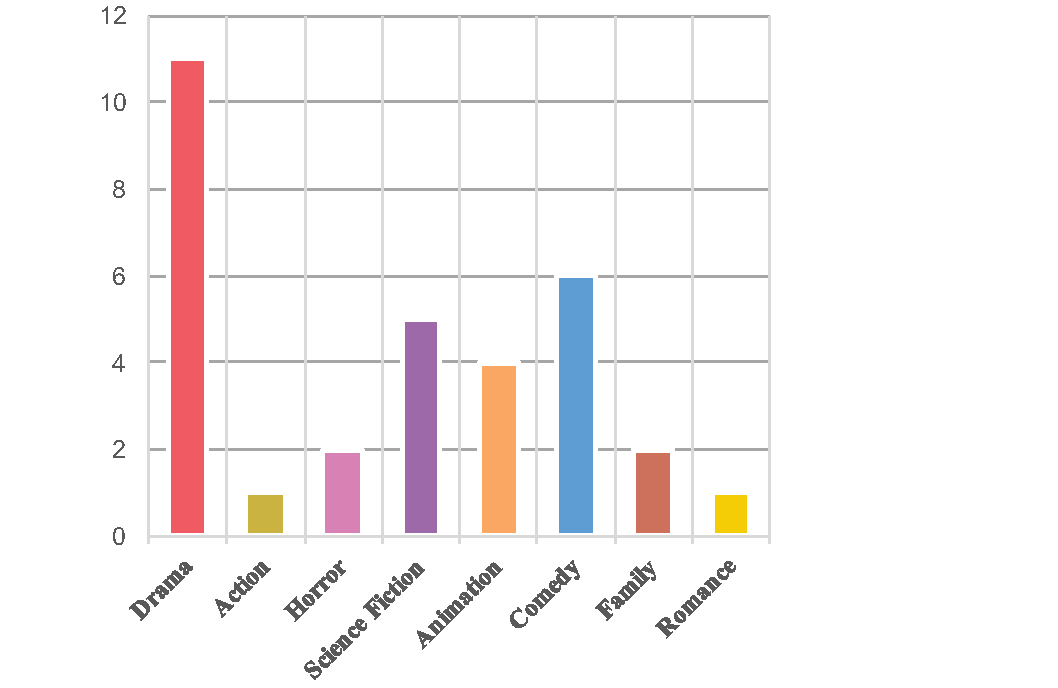
\includegraphics[width=10cm]{genre}
\centering
\caption{Distribution of genre in LIRIS-ACCEDE Dataset}
\label{genre}
\end{figure}

\begin{figure*}[h]
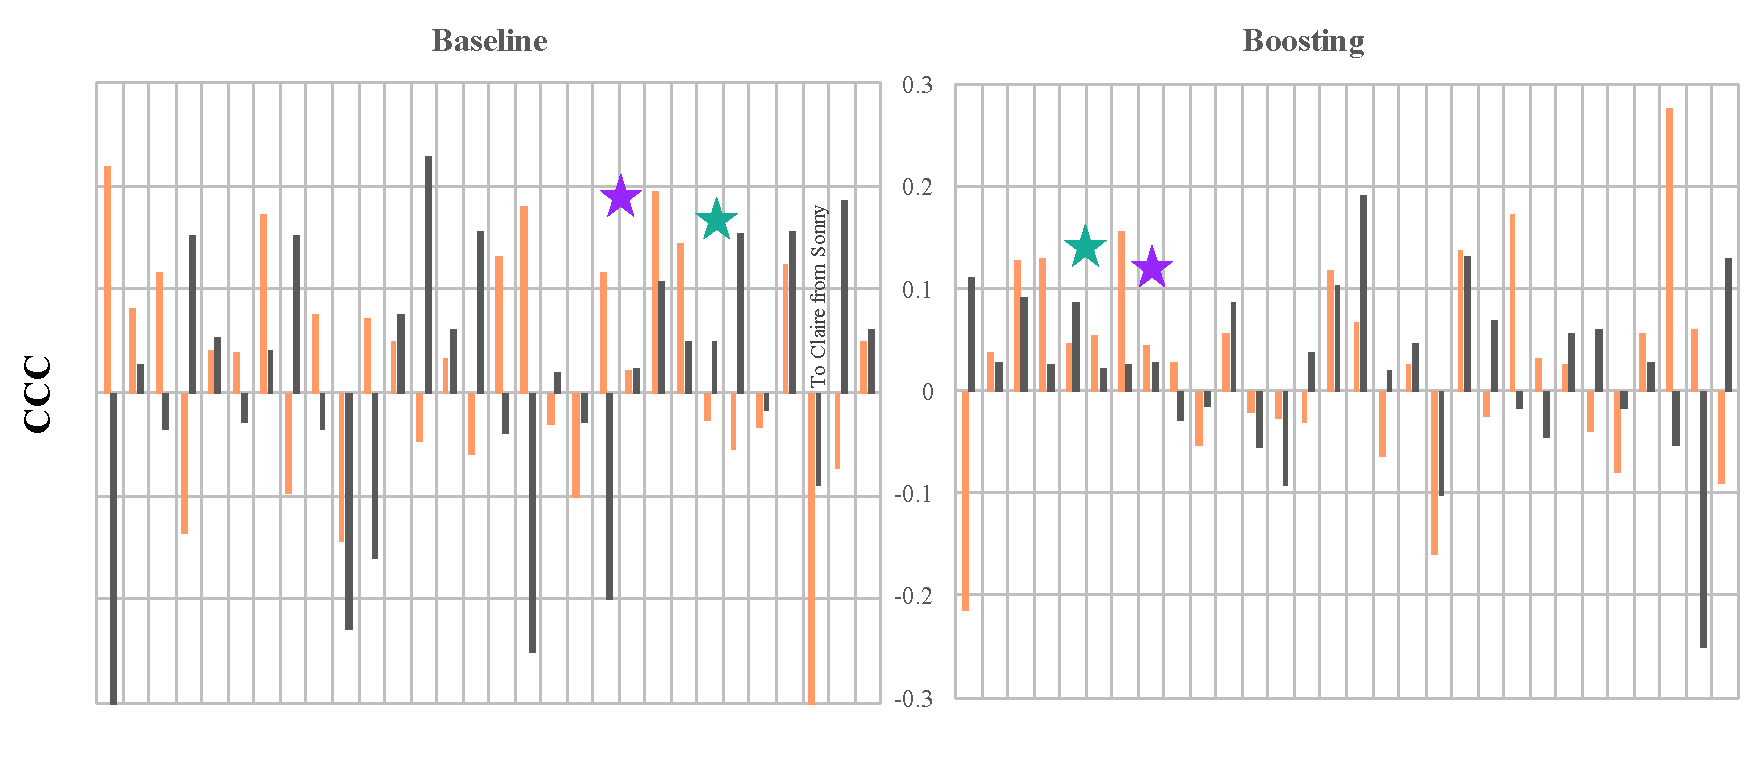
\includegraphics[width=\textwidth, height = 8cm]{comparison}
\centering
\caption{Performance of Baseline models and Gradient Boosting method across the 30 movies}
\label{comparison}
\end{figure*}

\subsection{Discussion}
We can observe the improvement in performance of Knowledge Transfer and Gradient Boosting compared to the baseline models. Among the baseline models, we observe that the linear models perform best for arousal, whereas neural networks show the best performance in valence prediction. There is no significant improvement for Gradient Boosting over Knowledge Transfer for valence prediction. When we analyze the performance farther across the movies, we observe a more consistent performance for both valence and arousal for gradient boosting compared to baseline. The case of the movie \textit{To Claire From Sonny} has already been discussed, and we can see the improvent in CCC after gradient boosting.

\section{Conclusion}
Knowledge Transfer from a larger and more varied dataset not only improves performance, but also results in more consistent CCC values for different movies. We have used root mean squared error as a proxy for the evaluation of pseudo-residual error for now. We endeavour to use CCC instead in the farther work. 

\footnotesize{
\begin{spacing}{.85 }
%\vfill\pagebreak
% BiBTeX files (here: strings, refs, manuals). The IEEEbib.bst bibliography
% style file from IEEE produces unsorted bibliography list.
% -------------------------------------------------------------------------
\bibliographystyle{IEEEbib2}
\bibliography{refs}
\end{spacing}
}
\end{document}
